\title{EE 393 Qs5}
% By default document is letter paper sized
\documentclass[11pt]{article}
% sets the margin to 1.0 inch
\usepackage[margin=1.0in]{geometry}
\usepackage{fullpage}
\usepackage[english]{babel}
\usepackage[utf8]{inputenc}
\usepackage{amsmath}
\usepackage{graphicx}
\usepackage[colorinlistoftodos]{todonotes}
\usepackage{array}
\usepackage{longtable}

\begin{document}
% 
\noindent
\Large \textbf{Alan Lee} \hfill 
\Large \textbf {EE-393 Technical Writing} \\
Quiz section AC \hfill Professor Bade \\
\today \hfill Kyle Lindgren

\begin{center}
\section*{Solar Powered Microgrids}
\end{center}

\section*{Problem Statement}


\section*{Solution}
With the use of solar panels and energy storage solutions, microgrids can be built that can supply electricity to the nearby inhabitants.

\section*{Project Specifications}

\begin{figure}[h]
\centering
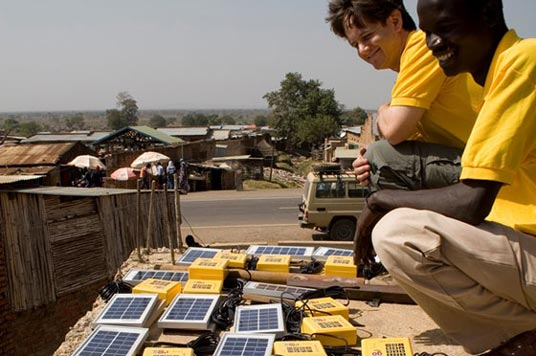
\includegraphics[scale = 0.20]{Solar_Panel.jpg}
\caption{}[h]
\end{figure}
\section*{Conclusion}
Improve the quality of life in the surrounding area while also 
\end{document}
